% !TEX root = ../zenkoku.tex
\section{結果}
熟練者がチームに1人いる状況を想定し,結果から熟練者への依存度が高いようなシステムを洗い出すことにした.
熟練者としては,アンケートの対象とする各サブシステムに直近1年間最も多くデプロイした開発者,新機能の実装やコードベースの管理に多く取り組んだ開発者,について総合的に判断し,当てはまる上位1人を今回の考察の対象とした.
またこれらの指標はOSS (Open Source Software) 開発プロセスに関する研究\cite{bib:mockus}におけるコア開発者の指標を参考にした.

アンケートの結果を\ri{img:rikai}に示す.

\begin{figure}[h]
	\centering
	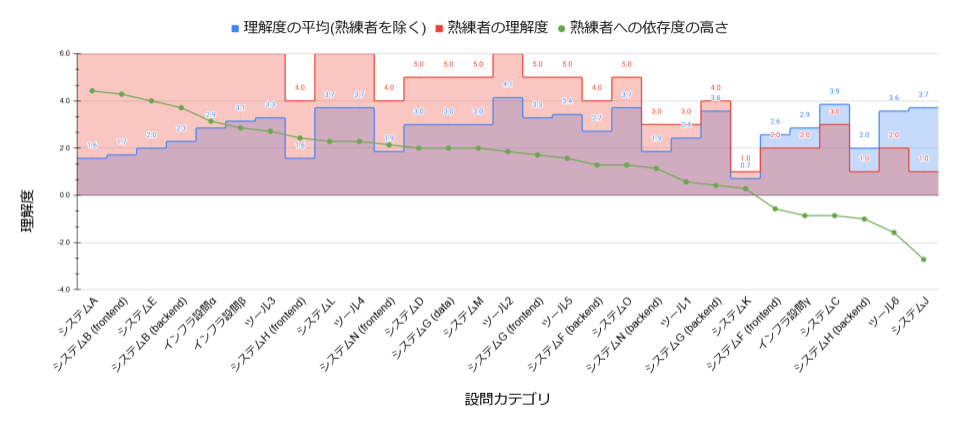
\includegraphics[keepaspectratio,width=0.9\linewidth]{img/rikai.png}
	\caption{理解度の平均と熟練者への依存度の高さ}
	\label{img:rikai}
\end{figure}

縦軸がブルーム・タキソノミーでの理解度,横軸が設問カテゴリ(各サブシステム)となっている.
また重ね合わせられている棒グラフは `熟練者の理解度 - 熟練者を除いた回答者の理解度平均` によって求めた理解度の差を表している.
各設問カテゴリの順番は左から熟練者への依存度の高い順に並べている.

また,この結果をアンケートを回答した開発組織のエンジニアに対し討論する機会を設けたところ,「この結果が示す理解度の平均・理解度の差,共に認識と相違ない」という意見が得られた.
